\documentclass[10pt,a4paper]{article}
\usepackage[utf8]{inputenc}
\usepackage{amsmath}
\usepackage{amsfonts}
\usepackage{amssymb}
\usepackage{a4wide} %Wider margins
\usepackage[english]{babel} %English dictionary for hyphenation and definitions, e.g. Table vs. Tabel
\usepackage[official]{eurosym} %Support for Euro-sign
\usepackage[utf8]{inputenc} %Support for internationalization, e.g. é vs.\’e
\usepackage{amsmath,amssymb,amsthm} %Support for mathematical formulas and symbols
\usepackage{fancyhdr} %Fancy headers
\usepackage{hyperref} %Creates clickable links
\usepackage{graphicx} %Support for grahpics
\usepackage{nopageno} %Support for removal of pagenumbers
\usepackage{tabularx}
\usepackage{enumitem}
\usepackage{xspace}
\usepackage{algorithm,algpseudocode}
\usepackage{float}
\usepackage{mathtools}
\usepackage[dvipsnames]{xcolor}
\usepackage[titletoc,toc,title]{appendix}
\usepackage{listings}
\usepackage{makecell}
\graphicspath{ {./ThesisFigures/} }

\hypersetup{
    pdftitle={}, %PDF-file will be given a proper title when viewed in a reader
    hidelinks %PDF-file will be given clickable, yet not visible links when viewed in a reader
}
\newcommand{\documenttitle}{Co-Morbidity in Bariatric Patients}
\newcommand{\documentsubtitle}{A new approach in quantifying the severity}


\newcommand{\true}{{\sc True}\xspace}
\begin{document}
	
	\begin{titlepage}
		
		\center
		
		\vspace*{3cm}
		
		\textbf{\huge \documenttitle}
		
		\textit{\LARGE \documentsubtitle}
		
		\vspace*{2cm}
		
		\large
		\centering
		T.P.A.~\textsc{Beishuizen}~(0791613)\\
		Biomedical Engineering - Computational Biology\\
		Data Engineering - Information Systems\\
		Eindhoven, University of Technology\\
		Email: \texttt{t.p.a.beishuizen@student.tue.nl}
		
		\vfill
		
		\vspace*{1cm}
		
		\today
		
	\end{titlepage}
	
	\tableofcontents
	
	%\newpage
	
	\pagestyle{fancy}
	%Abbreviations used by fancyhdr:
	%E Even page
	%O Odd page
	%L Left field
	%C Center field
	%R Right field
	%H Header
	%F Footer
	\fancyhead{} % clear all header fields
	\fancyfoot{} % clear all footer fields
	\renewcommand{\headrulewidth}{0.4pt}
	\renewcommand{\footrulewidth}{0.4pt}
	
	\fancyhead[L]{\rightmark}
	\fancyfoot[C]{\thepage}
	\fancyhead[R]{T.P.A. Beishuizen}
		
	\clearpage
	
	\section{Introduction}
	\label{sec:Intro}
	
	% Introduction Deneer's project
	Worldwide the number of bariatric surgeries is increasing. Although initially thought otherwise, this type of surgery has added benefits on top of losing weight, the primary reason. Among those benefits the remission of metabolic co-morbidities can be named. Due to binary labelling of those co-morbidities, valuable information is lost, while this labelling is not clearly defined either. To obtain more and better results, this binary labelling can be replaced by a continuous severity score. Ruben Deneer conducted a research on trying to achieve a successful replacement.\cite{Deneer2017Thesis}
	
	% First explanation data set
	The available data used for the research stemmed from the Catharina Hospital in Eindhoven (Subsection \ref{subsec:DataSets}). This extensive data set was a combination of two data sets and consisted of 41 markers measured pre- and post-surgery for 2367 patients that underwent gastric sleeve or gastric bypass surgery. These 41 markers are divided in several sub-panels that each describe different processes in the body. Conditions for these co-morbidities that were tested for the severity score were type II diabetes mellitus (T2DM), hypertension and dyslipidemia. Extensive literature research was done to connect them with 41 markers to find possible relations (Subsection \ref{subsec:CoMorMarkRel}). \cite{Deneer2017Thesis}

	% The goal of the research
	To better specify the research on the data, a main goal was created: \emph{to use data mining techniques to develop score that can objectively quantify the severity of co-morbidities present in bariatric patients based on biomarkers, both before and after surgery.} This means that it is not the goal to predict the outcome of the two types of surgery, but it is to quantify the improvement of the co-morbidities before and after the surgery. \cite{Deneer2017Thesis}

	% Layout Report
	Since the data is not available other than within the hospital, a figurative second study was conducted to complement Ruben Deneer's research. This study consists of three parts. The first part was creating a research question, hypothesis and an own analysis approach without the knowledge of Deneer's way. Since no data is available, this can only be made globally. It should be detailed enough, though, to compare it with Deneer's own approach. Secondly the two are compared and remarks are given on the original approach. At last both are combined to create a final proposal for a possible follow-up research. 
	
	\subsection{Data Sets}
	\label{subsec:DataSets}
	
	% Introduction + first data set
	Two data sets were used in the study. The first one is called "The Dutch Audit for Treatment of Obesity" (DATO). This data set is a national database that houses all registrations and health statuses of pre- and post treatment bariatric surgery patients in the Netherlands. Before surgery, the co-morbidities T2DM, hypertension and dyslipidemia were given a binary label of "Yes/No". After surgery they were given one of the following labels:
	
	\begin{enumerate}
		\item \textbf{Cured} No co-morbidity any more		
		\item \textbf{Improved} Less affected by co-morbidity
		\item \textbf{Same} No change in co-morbidity status
		\item \textbf{Worse} More affected by co-morbidity
		\item \textbf{Denovo} Diagnosed co-morbidity while not present before surgery
		\item \textbf{Not present} No co-morbidity present				
	\end{enumerate}

	% Second data set
	The second data set came from a laboratory database, stored in health records. This extensive data set consisted of 3 clinical and 38 blood markers measured pre- and 6, 12 and 24 months post-surgery. The tests pre-surgery had some additional markers on top of the 41 ones. These markers can be divided in the following categories: (Table \ref{tab:DataMarkers}) Complete blood count, liver function, kidney function, inflammation, lipid spectrum, coagulation, glucose metabolism, thyroid function and at last minerals and vitamins. The data sets of the patients that underwent bariatric surgery can be extracted from these. \cite{Deneer2017Thesis}
	
	\begin{table}
		\label{tab:DataMarkers}
		\caption{The markers present in the bariatric laboratory data set \cite{Deneer2017Thesis}}
		\begin{tabular}{lll}
			\hline
			~                     & Before Surgery/Pre-Op/Screening                                                                                                                     & After Surgery/Post-Op/Follow-up                                                                                                                     \\ \hline
			Complete blood count  & \makecell{hemoglobin\\hematocrit\\erythrocytes\\mean corpuscular hemoglobin\\mean corpuscular volume\\thrombocytes\\leukocytes}                                & \makecell{hemoglobin\\hematocrit\\erythrocytes\\mean corpuscular hemoglobin\\mean corpuscular volume\\thrombocytes\\leukocytes}                                \\ \hline
			Liver function        & \makecell{bilirubin\\aspartate aminotransferase\\alanine aminotransferase\\lactate dehydrogenase\\alkaline phosphatase\\gamma-glutamyltransferase}             & \makecell{bilirubin\\aspartate aminotransferase\\alanine aminotransferase\\lactate dehydrogenase\\alkaline phosphatase\\gamma-glutamyltransferase}             \\ \hline
			Kidney function       & \makecell{urea\\creatinine\\potassium\\sodium\\calcium\\phosphate\\albumin}                                                                                    & \makecell{urea\\creatinine\\potassium\\sodium\\calcium\\phosphate\\albumin}                                                                                    \\ \hline
			Inflammation          & \makecell{C-reactive protein}                                                                                                                                  & \makecell{C-reactive protein}                                                                                                                                   \\ \hline
			Lipid spectrum        &  \makecell{total cholesterol\\high-density lipoprotein-cholesterol\\total/high-density cholesterol ratio \\low-density lipoprotein-cholesterol \\triglycerides} & \makecell{total cholesterol\\high-density lipoprotein-cholesterol\\total/high-density cholesterol ratio \\low-density lipoprotein-cholesterol \\triglycerides} \\ \hline
			Coagulation           & \makecell{prothrombin time}                                                                                                                                    & \makecell{prothrombin time}                                                                                                                                   \\ \hline
			Glucose metabolism    & \makecell{hemoglobin A1c (IFCC)\\glucose\\insulin\\C-peptide}                                                                                                  & \makecell{hemoglobin A1c (IFCC)\\glucose\\-\\-}                                                                                                                \\ \hline
			Thyroid function      & \makecell{parathyroid hormone\\thyroid-stimulating hormone\\free T4\\cortisol}                                                                                 & \makecell{parathyroid hormone\\-\\-\\-}                                                                                                                        \\ \hline
			Minerals and vitamins & \makecell{iron\\ferritin\\folic acid\\zinc\\magnesium\\vitamin A\\vitamin B1\\vitamin B6\\25-OH vitamin D\\vitamin B12}                                        & \makecell{iron\\ferritin\\folic acid\\-\\-\\-\\vitamin B1\\vitamin B6\\25-OH vitamin D\\vitamin B12}                                                           \\ \hline
		\end{tabular}
	\end{table}
	
	% Data comibining challenge one
	A smaller part of the research is to combine these two data sets. Some challenges arise when doing so. Such a challenge is obviously to find the right connection between them, using the survey and lab data of the same patient. What can the markers say about the severity of co-morbidities?
	
	% Data driven challenge two
	A second challenge would be to define what to do with non-matching data. In the pre-treatment for example more markers were used than in the post-treatment. These missing ones might be more useful for scoring the co-morbidity severity than the known markers. There also might be measurements that were missing or corrupted, whereas other markers might still be useful enough for a result. How to tackle this missing data challenge should be defined properly.
	
	\subsection{Co-morbidity Marker Relation}
	\label{subsec:CoMorMarkRel}
		
	% Introduction section
	For some of the markers it is clear they affect the severity score of a co-morbidity. Co-morbidity is diagnosed from this markers and therefore a relation is imminent. For others more subtle relations are present, that in first sight would not be recognised. Both are important for assigning a co-morbidity severity score.
	
	% Clear relations
	All three co-morbidities can be derived from specific markers. T2DM is known for higher glucose and insulin levels in the blood, while hardly finding any C-peptides. Ideally these would be used to find T2DM, however these values vary significantly over the day. Therefore help from other markers should be helpful. Hypertension is best measured with blood pressure measurements (BP). These however are not reliable for the nervous patients in the hospital and other markers must be found for help. Thirdly dyslipidemia obviously can be found using markers in the lipid spectrum (Table \ref{tab:DataMarkers}), however there may be other markers contributing to dyslipidemia detection, as well.\cite{Deneer2017Thesis}
	
	% Less well-known relations
	For T2DM, hypertension and to a lesser extend dyslipidemia, more knowledge on relations between them and markers would benefit the creation of a severity score. Literature research is done to understand more of those subtle relations and know that those exist when trying to create a morbidity score. The outcome of this literature search shows that quite some relations can be found between co-morbidities and the markers (Table \ref{tab:CoMorMarkRel}). For most it is definitely worth to investigate any relation.\cite{Deneer2017Thesis}
	
	\begin{table}[]
		\centering
		\caption{Relations found in literature between the co-morbidities and markers.\cite{Deneer2017Thesis}. The number shows how many citations were found that state a relation exist, nothing means no relation. A 'D' means that the disease is diagnosed from those markers.}
		\label{tab:CoMorMarkRel}
		\begin{tabular}{llll}
			\hline
			& \textbf{Diabetes} & \textbf{Hypertension} & \textbf{Dyslipidemia} \\ \hline
			hemoglobin            & 3                 & 1                     &                       \\
			hematocrit            & 2                 & 2                     &                       \\
			erythrocytes          & 1                 & 1                     &                       \\
			MCH                   &                   & 1                     &                       \\
			MCV                   &                   & 1                     &                       \\
			thrombocytes          &                   &                       &                       \\
			leukocytes            & 4                 & 3                     & 1                     \\
			bilirubin             & 3                 & 1                     & 1                     \\
			ASAT                  & 1                 & 1                     & 1                     \\
			ALAT                  & 4                 & 1                     & 1                     \\
			LD                    & 1                 &                       &                       \\
			Alkaline phospatae    & 2                 &                       &                       \\
			gamma GT              & 4                 & 2                     & 1                     \\
			urea                  & 1                 & 3                     &                       \\
			creatinine            &                   & 2                     & 1                     \\
			potassium             &                   & 2                     &                       \\
			sodium                &                   & 1                     &                       \\
			calcium               & 2                 & 1                     & 1                     \\
			phosphate             &                   &                       &                       \\
			albumin               &                   &                       &                       \\
			CRP                   & 3                 & 4                     & 1                     \\
			cholesterol           &                   & 2                     & D                     \\
			HDL-cholesterol       &                   & 2                     & D                     \\
			chol/HDL ratio        &                   &                       & D                     \\
			LDL-cholesterol       &                   & 2                     & D                     \\
			triglycerides         &                   & 2                     & D                     \\
			prothrombin time      &                   &                       &                       \\
			hemoglobin A1c (IFCC) & D                 &                       &                       \\
			glucose               & D                 & 2                     &                       \\
			parathormone          & 1                 & 2                     &                       \\
			iron                  &                   &                       &                       \\
			ferritin              & 3                 & 1                     & 1                     \\ \hline
		\end{tabular}
	\end{table}
	
	\clearpage
	
	\section{First Proposal}
	
	% Research question
	To start of a research proposal, the first thing that needs to be done is to create a research question that fits the intended goal. This main question can then divided in several sub questions for explaining the steps how to answer it. Next hypotheses should be made for the main and sub questions. Thirdly the methods of how to answer the research questions are discussed. 
	
	\subsection{Research Questions}
	
	% Main question
	As stated earlier (Section \ref{sec:Intro}) the goal was to develop a severity score for the co-morbidities using data mining. A research question for this goal would then be:
	
	\begin{enumerate}
		\item[] \emph{Can a severity score for co-morbidities present in bariatric patients based on biomarkers be developed?}
	\end{enumerate}
	
	% First sub-question
	This main research question includes all aspects of the goal. It can however be specified in several different sub-questions. A first sub-question would be about the relation between the co-morbidities and the biomarkers, which is a major part on making this score.
	
	\begin{enumerate}
		\item \emph{Which relations are present between co-morbidities and the biomarkers?}
	\end{enumerate}
	
	% Second sub-question
	A second sub-question should be about retrieving the score for the co-morbidities from the biomarkers. This score retrieval should use the outcome of the first sub-question to efficiently find the correct score.
	
	\begin{enumerate}[resume]
		\item \emph{How can a severity score of co-morbidities be obtained from biomarkers?}
	\end{enumerate}
	
	% Explanation relation both questions to main
	This second questions mainly focuses on techniques to achieve a sufficient answer to the main research question. When both sub-questions are sufficiently answered, then the main one should definitely be, as well.
	
	\subsection{Hypothesis}
	
	% Pre-conditions
	The data set available for this research is quite extensive. The number of biomarkers is high, many relations between them and the co-morbidities are known and a high number of patients has been tested for both. These pre-conditions are very beneficial to finding positive answers for the research questions.
	
	% First sub-question
	Knowing many relations between the co-morbidities and biomarkers beforehand implies that a lot of them should be present in the data set. to the first sub-question which relations are present, the answer would be two-fold. First strong relations between the co-morbidities and on the other hand biomarkers that help diagnosing them. This would for example be the case for dyslipidemia and biomarkers of the lipid spectrum. Weaker relations are expected for all found in literature (Table \ref{tab:CoMorMarkRel}).
	
	% Second sub-question
	As for the second sub-question how a score can be defined from biomarkers, several different options are possible. When knowing there is a relation between biomarkers and the co-morbidity, with machine learning combined with regression a function can be made predicting a score outcome for the biomarkers. This score is then compared with the categorical labelling of co-morbidities to find out if they match. This way, through training the model and afterwards testing if that model could efficiently give a good score to the co-morbidities.
	
	% Main research question
	With the hypotheses for both sub-questions the main research question can be answered, too. The hypothesis for this one would be that it is possible to find a severity score with the biomarkers. A model can made using the biomarkers as an input and retrieving a severity score as output.
	
	\subsection{Methods}
	
	% Materials
	Since the materials are all explained in Deneer's thesis, that part and most of the pre-processing is skipped in methods. One thing that needs to be discussed is the handling of markers that are measured pre-surgery, but not post-surgery. These could be removed as being redundant. They may, however show a significant difference between availability or absence of a co-morbidity. This is a vital result for possible further bariatric surgeries and co-morbidity scoring. Therefore at least some tests should be done with those pre-surgery biomarkers. For post-surgery measurements they can be removed from the tests or they can be given a dummy value as being unknown.
	
	% Methods first sub-question
	The first research question can be easily and efficiently answered with statistical analysis. This approach can be used to compare two groups of values, whether the co-morbidity is present or not. Since for this question a score is not yet needed, dividing the patients between having a co-morbidity and not suffices. The markers that show a significant difference in mean or in variance should be noted and given extra care in future researching to create a score. Aside from comparing original measurements of the markers, combinations between them should be tested for statistical analysis as well. Some are already present, for example the \textit{cholesterol / HDL-cholesterol ratio}. There may be more interesting combinations that could show a significant difference for either of the three co-morbidities.
	
	% Program first sub-question
	Since the data needs some manipulation to find those markers that are significantly different for presence or absence of co-morbidities, a more advanced statistical program that can do those manipulation would be best to use. This means that the best choices would be R, MATLAB or Python. Python was chosen of those three for also being a good choice for researching the second sub-question and because the actual users knows Python quite well. The outcome of this research can most likely immediately used in the second one for the next sub-question
	
	% Program second sub-question
	The second research question is a bit more complex to answer. The quickest one is to use a way of machine learning to create this score. Some sort of regression is the first thing that comes to mind and simple support vector machines (SVMs) seem to be a good way to start. However obtaining a continuous score from categorical, or in the case of pre-surgery even binary, labels. A score interval needs to be set up and these binary or categorical values should be translated to a certain score on the interval. The way to score these values can be proposed, but most likely needs more insight to find out what is best. At first just a categorical learning system seems best. Both a selection of from sub-question resulting useful markers should be used as well as the complete set to find a good score.
	
	% At the start a score interval of 0\% to 100\% will be chosen, with 0\%-50\% being not having the disease and 50\%-100\% having it, with different severities. Binary cases will then be given 25\% and 75\% as absent and present co-morbidity respectively, knowing those as the values they should be closest to. The ordinal cases that showed improvement or deterioration will be given a score of 50\%. 
	
	% Program second sub-question
	At the start of researching this second sub-question a standard machine learning framework would suffice. This means that the aforementioned Python with the Scikit-learn package would be best to start with. When initial results indicate that a certain way of handling this data in another way would be more efficient, Python is used by many other machine learning programs, such as Theano, TensorFlow and both their packages. Therefore Python would be a great way to start the project of which the direction can change heavily.
	
	\clearpage
	
	\section{Original research}
	
	% Introduction original research
	Now that an initial proposal is made, the original research should be discussed. This original research is divided into two parts. The first part is all about the material and how this was preprocessed. The second part focused more on modelling using the data sets. Multiple approaches have been used to show different aspects of the data.
	
	\subsection{Preprocessing}
	\label{subsec:Preprocessing}
	
	% Merging data sets
	As discussed earlier (subsection \ref{subsec:DataSets}), the data is retrieved from two data sets, the DATO and lab set. These two are not perfectly lined up and therefore merging those required some specific rules. At first, any entries that were double on the same date were removed as they had conflicting information. Entries that had surgery before 2012 were removed, too, due to not having a pre-screening test. Secondly all DATO and lab sets were paired up if they did not have more than 90 days between them. When double matches occur, the closest ones were taken. Also only pairs were taken when they were on on of the four periods (pre-, 6, 12 or 24 post-surgery) and others were omitted.
	
	% After merging preprocessing
	After merging both data sets the lab data was prone to preprocessing. Ten biomarkers were dropped from the set, due to missing values. Five (Zinc, vitamin A, free T5, methylmalonic acid, LDL) were dropped due to severe missing data or explained by other data. Five others (TSH, insulin, C-peptide, magnesium and cortisol) were dropped due to only being available in pre-surgery screening. CRP is dichomotized, due to being truncated and comparable results are made their cut-off value, due to only a small portion of results being affected by that. Inconsistencies in DATA meant that that patient would be dropped. After all these markers being removed, a total of 60 variables are present in the data set (figure \ref{fig:FinVar}) and a number of 2367 patients with a 2.35 of data sets per patient on average (figure \ref{fig:FinPat}). The number of variables used for modelling is reduced to 49. From those, a nunber of variables are removed again. Weight and height (incorporated in BMI), vitamins (are supplemented), iron (variation too high), year, type of and months before/after surgery (no value, or found elsewhere) are all removed. Furthermore Creatinine is replaced by glomerular filtration rate (GFR), the ASAT/ALAT ratio was added, the prothrombin time (PT) is replaced by the international normalized ratio (INR) and at last calcium is corrected by adding an albumin factor. 
	
	\begin{figure}
		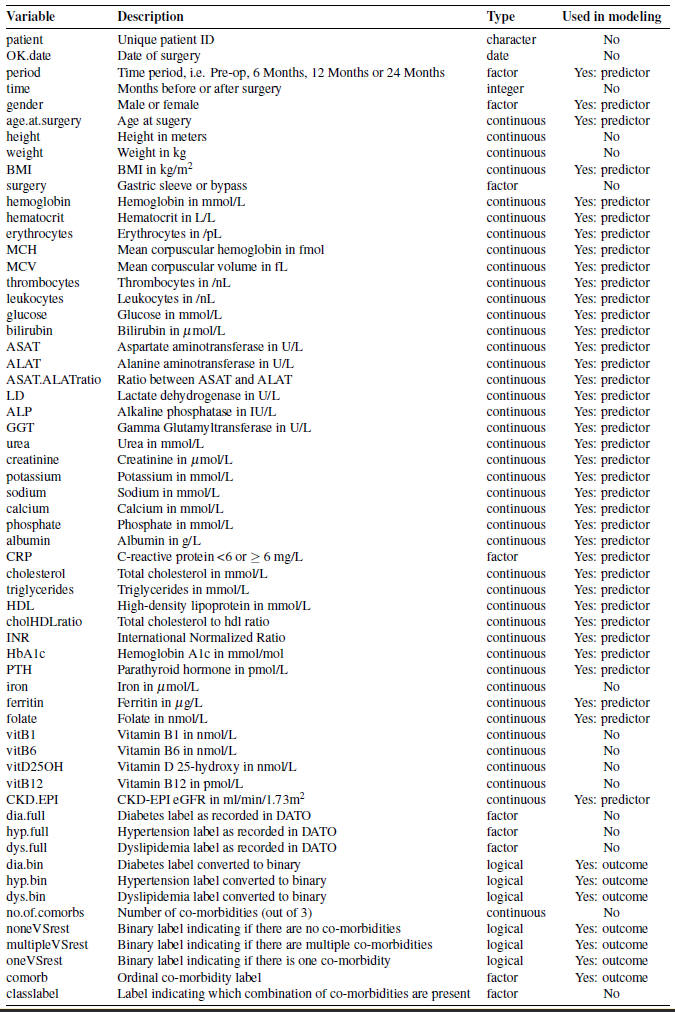
\includegraphics[scale=0.8]{FinalVariables.PNG}
		\label{fig:FinVar}
		\caption{All variables present after pre-processing \cite{Deneer2017Thesis}}
	\end{figure}
	
	\begin{figure}
		\includegraphics[scale=0.8]{FinalPAtients.PNG}
		\label{fig:FinPat}
		\caption{All patients present after pre-processing \cite{Deneer2017Thesis}}
	\end{figure}
	
	\subsection{Modelling}
	
	% Modelling layout
	After preprocessing the data, a series of steps should be taken to create a sufficient model for the issue. First an ordinal outcome definition is made for scoring the co-morbidities. Next, statistical learning models are created, based on logistic regression and all aspects of this model are discussed to find, validate and visualize a correct model.
	
	% Ordinal outcome
	To make one scale for all co-morbidities a new ordinal outcome was created. This scoring was made with three different categories, being no, one or multiple co-morbidities present. The choice for this scoring was made with the idea that people with more co-morbidities also have a higher severity of them compared with patients that have less or none. Multiple co-morbidities was a merge from having two and three, due to making the categories more balanced in size. This way none has most patients (1329) and one and multiple still have a decent number (569 and 469 respectively). 
	
	% Statistical models
	To create a model in this research, a classification method should be used. A well known one for that is logistic regression. Maximum likelihood estimation is used to estimate regression coefficients for the variables. Multicollinearity must be limited as much as possible, as it is assumed to be absent for logistic regression. A correlation matrix is created to find multicollinearity. Special interactions are included as well, for example the Body mass index (BMI) and presence for co-morbidities as being a prerequisite for the surgery. For ordinal outcome of the logistic regression, both proportional odds (PO) as continuation ratio (CR) were used. 10-fold cross validation was done to validate the model and an assessment of model fit was done for discrimination, calibration and overall performance. Lastly the model is visualized with a nomogram, for further use.
	
	\clearpage
	
	\section{Proposal Comparisons}
	
	% Introduction propposal comparisons
	A proposal is created after reading the introduction, background and material. The original research is also discussed and a summary is given. This new proposal should now be compared with the original research to find out when they match and when they have different approaches. Several topics should be discussed that differ greatly between the original and new proposal. This differences need to be addressed to create a final proposal for a possible new research. The first difference is about data  omission. Many aspects of the original data set are debatable whether they should be removed or not. A second difference is the final scoring system. The newly proposed one is vastly different then the original one.
	
	\subsection{Data Omission}
	
	% Data omission locations
	In preprocessing (subsection \ref{subsec:Preprocessing}) a big number of data omissions is done due to various reasons. While there are many regarded as valid, a number of them can be seen as being a bit too rigorous. These questionable ones are discussed whether they should be left out.
	
	\begin{enumerate}
		\item \textbf{lab set without close DATO set} Several lab sets were removed because no DATO set was close enough. This seems logical as they should match for complete results. However the DATO set has many variables that are not subject to much change over time. If a lab set is squeezed in between DATO sets that are very similar, an estimate for the intermediate DATO set at that time could easily be made.
		
		\item \textbf{Predefined measuring moments} The DATO and lab sets were all measured on predefined moments. There were other times as well, though, were they were measured. On those other times the data was omitted. These omissions are too rigorous. These data sets are maybe not useful enough to show differences on those measuring moments, however this data could be very helpful to create a model. These questionable omissions include pairs that were double on one moment and the ones on 36 or 48 months. 
		
		\item \textbf{Markers only in pre-surgery measurements} Five of the biomarkers were only measured in before the surgery. The reason for this is not stated, however these markers are removed as only about half of the data sets have these. When almost 50\% of the data sets have these markers, there is enough available to check these variables on their relation with the co-morbidities. If all of them show no significant difference in presence or absence of the co-morbidities, then they are not useful. If they do show a significant difference, they might be a good marker for further co-morbidity detection. Disregarding them only because half of the sets don't have the value seems questionable.
		
		\item \textbf{LDL-cholesterol} This marker from the lipid panel was removed due to the possible derivation of it from the same panel markers. The omission is discussed quite heavily in the thesis. Even though it is derived from other markers, the derivation is done in a specific way. Maybe a description for one of the co-morbidities would benefit greatly of this specific derivation. Even though this is the weakest of cases where omission is questionable, at least some tests could be done to check the significance.
		
	\end{enumerate}
	
	\subsection{Scoring System}
	
	% Difference scoring system
	At the project start a goal was made about creating a severity scoring system for co-morbidities. To achieve this goal of creating a score from categorical data, as little data reduction as possible should be done to keep the score quality as high as possible. The proposed ordinal system however actually reduces information. There is no distinction between two or three co-morbidities. The type of co-morbidity is removed, too, as well as its progress after surgery. This is a very counter intuitive way to correctly model a scoring system when these three decisions all could contribute to more efficient scale.
	
	% Final scoring system
	The final scoring system is not really an answer to the original goal. This was to create a severity score, whereas the linear predictor score in the nomogram is originated from its probability counterpart and not really showing severity. As discussed earlier, it is hard to create a severity score from categorical labelling, so maybe this goal might be too ambitious. Using predictability score is a straightforward start for this, though, as those can be calculated. Further research may lead to a severity score from that. 
	
	% Better proposal
	For this research it seems better to keep the three co-morbidities separate as long as possible. For every co-morbidity separately a score could be made which in the end can be joined together. This score would at start be best based on a probability, so how much chance there is to have a certain co-morbidity. After creating probability models for all of them, they can be combined in a joint probability model. When doing this obviously collinearity needs to be taken into account. 
	
	% Not according to goal
	A probability model is not according to the goal though, as a score was wanted and not a probability. Since the data is not gathered in a way to find a score with the measured tasks, this is much harder. After possibly finding a good results for a probability model, a next step could be to translate that model in a scoring system.
	
	\subsection{Modelling Tools}

	% Used modelling tools
	About every part of the original research is done in R. As discussed previously, especially the variable significance can be done efficiently in R, as it is one of the more advanced tools to do statistical analysis. For the modelling part however there are more advanced programs or frameworks that can be used. One of the reasons for this was to create a "white-box" answer, that every step of the process can be explained. The disadvantage in choosing a white-box model, however, is that the result can be worse than for a more traditional machine learning approach. Those approaches could lead to a better result and are therefore definitely worth to investigate. In R however, machine learning options are extremely limited if even available. Other programs or frameworks could facilitate that better than R, such as python, the Scikit-learn package, Theano or Tensorflow. This could also facilitate a better final visualization result for the scoring system than the nomogram, which is not very user-friendly and straightforward.
	
	\clearpage
	
	\section{Final Proposal}
	
	% Introduction final proposal
	The final proposal combines the first one and the original research for optimization. The research questions from the first proposal are re-used, with some modifications and additions. The hypotheses are changed accordingly. The methods for answering the research questions are similar to the ones in the first proposal, however, they are extended after more information from the original research is added. 
	
	\subsection{Research Questions}
	
	% Main research question
	The main research questions stays the same as the main one of the first proposal. This is the main goal of the research and therefore is a good all-encompassing question for it. 
	
	\begin{enumerate}
		\item[] \emph{Can a severity score for co-morbidities present in bariatric patients based on biomarkers be developed?}
	\end{enumerate}
	
	% First sub-question
	The first sub-question also stays mostly the same. It was a bit unclear that there was relevant data in the DATO set. Therefore instead of saying biomarkers, the term "available variables" will be used. The word available is added due to not immediately omitting some of the variables, so their relation to co-morbidities is still investigated.
	
	\begin{enumerate}
		\item \emph{Which relations are present between co-morbidities and the available variables?}
	\end{enumerate}
	
	% Addition to first sub-question
	One thing the original research correctly investigated that was not thought of, was collinearity. This was already investigated for most variables, however the ones then removed might still have collinearity characteristics. Therefore a new sub-question is added to find those characteristics.
	
	\begin{enumerate}[resume]
		\item \emph{Which collinearity relations are present within the available variables?}
	\end{enumerate}
		
	% Second sub-question I
	The other sub-question was about adding a score to the co-morbidities with the variables. This question was quite vague and with the help of the original research it is split up in three separate questions. The first one is about modelling the co-morbidities with variables.
	
	\begin{enumerate}[resume]
		\item \emph{How are the co-morbidities best modelled with the available variables?}
	\end{enumerate}
	
	% Second sub-question II
	The second part of the split sub-question is about the scoring part. Eventually a score should be given to the co-morbidities, which  must be investigated thoroughly.
	
	\begin{enumerate}[resume]
		\item \emph{How can scores best be added to the available co-morbidity models?}
	\end{enumerate}
	
	% Second sub-question III
	The last part is about combining the co-morbidities together. Until now they are regarded separately, but the eventual result should have these scores combined. Therefore the third one of the split sub-question is about combining those.
	
	\begin{enumerate}[resume]
		\item \emph{How can the co-morbidity models best be combined?}
	\end{enumerate}
	
	% Final thoughts
	This main question and the five sub-question should cover all aspects in this research. If all questions are answered, one by one, a scoring model for the co-morbidities should be available for bariatric patients.
	
	\subsection{Hypotheses}
	
	% Introduction Hypothesis
	Since three sub-questions are added. The new hypotheses should be added, as well. They will be addressed in order of appearance and afterwards a general hypothesis will be given for the main research question.
	
	% First sub-question
	The first sub-question has the same hypotheses as in the earlier proposal. Strong relations should be found in the markers that the co-morbidities are diagnosed from and weak relations should be found in the ones that are linked in literature. On top of that, since the original research answered this question partially, too, the following variables should show strong relations: triglycerides, HbA1c, CKD.EPI, age.at.surgery, HDL, cholesterol0-HDL-ratio, albumin, period, potassium, period * BMI, cholesterol and urea. All of these showed the best correlation.
	
	% Second sub-question
	The second sub-question has also been partially answered in the original research. Therefore strong relations should be found between: hematocrit and hemoglobin, MCV and MCH, ALAT and ASAT, HbA1c and glucose, hemoglobine and gender, erythrocytes and hematocrit. Aside from these mostly the omitted variables should show relations within their own panel. Insulin for example is expected to show a relation with glucose and C-peptide.
	
	% Third sub-question
	The third sub-question is partially answered in a specific direction by the original research. Logistic regression was extensively investigated, however other machine learning aspects were not used. The hypothesis is that most likely several machine learning methods should be sufficient to answer this question. With those machine learning methods a model can be derived for the co-morbidities to be found out of the available variables.
	 
	% Fourth sub-question
	The fourth question is the also hardest. How can a score be added? The original research started first with an ordinal score, which is debatable for the information thrown away. When thinking ahead, the best idea for now is to start with a probability score. These probabilities usually also show the severity, as having a higher probability for a co-morbidity, the severity of it usually is bigger, too. After having a probability score further insights can be used to create a better score than probability. An example of such a score can be this:
	
	\begin{enumerate}
		\item[] \textbf{Score proposal} At the start a score interval of 0\% to 100\% will be chosen, with 0\%-50\% being not having the disease and 50\%-100\% having it, with different severities. Binary cases will then be given 25\% and 75\% as absent and present co-morbidity respectively, knowing those as the values they should be closest to. The ordinal cases that showed improvement or deterioration will be given a score of 50\%. 
	\end{enumerate}
	
	% Fifth sub-question
	The last sub-question is bigger than only adding them together. Since the co-morbidities are also related to each other, these correlations have to be taken into account when creating a score. On the other side, when two co-morbidities are both present in a patient, they also have a bigger chance to be more severe, as they strengthen each other. Different additions or combinations can be tested to combine them.
	
	% Main research question
	The hypotheses of most sub-questions are fairly straightforward and with the original research are known to give results already. The aim is however to create better answers than the already available ones. For the first two questions this is definitely possible, the last three depend whether the results will be improving the known ones already, mainly because it is a new area for researching. Still, though, as there is already one present, the main research question can be answered with a yes.
	
	\subsection{Methods}
	\label{subsec:FinalMethods}
	
	% Introduction methods
	This time the methods is changed a bit from the first proposal, as it would be better to line them up with the original research and show differences between those. So first we start with the preprocessing and every thing that is related to that. Secondly the modelling part will be discussed, together with the sub-questions that are answered in here.
	
	% Preprocessing
	In preprocessing almost every thing will be done the same as in the original research. Most differences will be in not removing certain parts of the data set. This means that more than one data set can be made for the different instances. All differences will be discussed.
	
		\begin{enumerate}
		\item \textbf{All paired DATO and lab set} All data that is available after pairing the DATO and lab set will be put in a data set. There will not be any distinction between data on predefined moments and not, because for modelling those do not matter at all. I case more results should be generated on those predefined moments, a separate attribute set will be made.
		
		\item \textbf{Variables omission} Not all variables will be omitted when a significant number of them is available. Relations between those variables and with the co-morbidities will be tested. When finding out that there are significant relations between them, possible further research will be done on both a set with and without them. Variables that fall into this category are the five that are only measured pre-surgery and LDL.
		
	\end{enumerate}
	
	% Modelling layout
	Several steps should be taken to achieve the final goal. First the variables needs to be compared with the co-morbidities (sub-question 1) and themselves (sub-question 2). Next a model has to be found (sub-question 3) for all co-morbidities as well as a score added to the model (sub-question 4). Lastly the three models need to be combined (sub-question 5) to create a final answer to the main research question.
	
	% Variable exploration
	To answer the first two sub-questions, statistical analysis must be done. Correlation matrices must be made to see whether two variables or one and a co-morbidity correlate significantly. Also the variables must be checked on their own population, whether they have a high variance and follow a statistical distribution. In case of high correlations between variables, a joint variable should be created if possible. At last, also combinations of variables should be created and tested for relations with co-morbidities. This all can efficiently be done in Python with the SciPy package.
	
	% Co-morbidity modelling
	A co-morbidity can be modelled using different approaches in machine learning. Several classification techniques are available such as support vector machines (SVM), nearest neighbour (NN), stochastic gradient descent (SGD). Research must be done which is most applicable and testing must be done which gives the best results. This is repeated three times for every co-morbidity. Within Python the Scikit-learn package has the basics to create proper results and if needed, programs such as Theano or TensorFlow can be added. For testing, a similar approach as in the original result can be used, 10 fold cross-validation. The final model and the visualisation depends on the type of machine learning used, however graphs that show clusters of morbidities for several variables seems a good way to approach that.
	
	% Co-morbidity scoring
	To add scoring in machine learning approaches is a challenge. At first tests can be done with changing the methods from classification approach to their regression counterpart, for example from SVC (Support Vector Classification) to SVR (-Regression). This can have major for now unknown implications. As discussed earlier (subsection \ref{subsec:FinalMethods}) setting up a score interval should be thought of before and also able to be implemented. The proposed score can be used as a base and be changed if advantageous.
	
	% Co-morbidity combination
	The last challenge is to create a model that combines all three of the co-morbidities. To start this, all three separate models can be used to create the combination. If this does not give the desired results and makes scores much worse than initially thought, a similar ordinal system as used in the original approach can be used. Then sub-questions three and four are repeated only with co-morbidities combined, removing details from each different one.
	
	\bibliography{Citings} 
	\bibliographystyle{ieeetr}
	
\end{document}
